\documentclass[ASNA,twocolumn]{USG}
\usepackage{anyfontsize}
\usepackage{amsmath}
\usepackage{booktabs}
\usepackage{array}
\usepackage{etoolbox}
\usepackage{microtype}
\graphicspath{{./figures/}{./images/}}

% Retain the supplied class and author metadata; remove sample-journal branding.
\makeatletter
\patchcmd{\@maketitle}{\includegraphics[width=56mm]{allergy.eps}}{}{}{\errmessage{Sample logo patch failed}}
\patchcmd{\@maketitle}{\vskip24.36mm}{\vskip7mm}{}{\errmessage{Title spacing patch failed}}
\patchcmd{\@@articletype}{\includegraphics[width=0.70in]{images/openaccess}}{}{}{\errmessage{Sample access badge patch failed}}
\let\@history@dates\@empty
\makeatother
\raggedbottom
\pagestyle{plain}
\floatpagestyle{plain}
\rotfloatpagestyle{plain}
\setcounter{topnumber}{3}
\setcounter{dbltopnumber}{2}
\renewcommand{\topfraction}{0.90}
\renewcommand{\dbltopfraction}{0.90}
\renewcommand{\textfraction}{0.08}
\renewcommand{\floatpagefraction}{0.75}
\renewcommand{\dblfloatpagefraction}{0.75}
\setlength{\emergencystretch}{1em}

\articletype{ORIGINAL ARTICLE}
\journal{International Journal of Circuit Theory and Applications}
\articledoi{}
\volume{}

\begin{document}
\title{FCNPilot: A Tool-Grounded Agentic Framework for End-to-End Field-Coupled Nanocomputing Circuit Design}
\author[1]{Yangshuai Li}[https://orcid.org/0000-0001-5060-9621]
\author[1]{Hao Xiao}[https://orcid.org/0009-0004-6419-9984]
\author[1]{Qian Han}[https://orcid.org/0000-0002-7171-134X]
\author[2]{Fei Peng}[https://orcid.org/0000-0002-2835-0120]
\author[1]{Guangjun Xie}[https://orcid.org/0000-0002-7801-2875]
\authormark{LI \textsc{et al.}}
\titlemark{FCNPilot: Agentic FCN Circuit Design}
\address[1]{School of Microelectronics, Hefei University of Technology,
Hefei~230601, China}
\address[2]{School of Computer Science and Technology, Hebei Finance University,
Hebei~071051, China}
\corres{Yangshuai Li (\email{2023010123@mail.hfut.edu.cn}) ~|~
Hao Xiao (\email{xiaohao@hfut.edu.cn}) ~|~
Qian Han (\email{hq85689241@163.com}) ~|~
Fei Peng (\email{fpeng1985@126.com}) ~|~
Guangjun Xie (\email{gjxie8005@hfut.edu.cn})}
\keywords{field-coupled nanocomputing | quantum-dot cellular automata | physical design | Boolean equivalence | large language models | design automation}
\abstract[ABSTRACT]{\textbf{Objective:} Language-guided circuit design requires a distinction between successful tool execution and a valid circuit representation. This work studies that distinction for combinational field-coupled nanocomputing circuits.
\textbf{Methods:} FCNPilot, a Pi-based domain agent, connects scalar Verilog, routed directed acyclic graphs, clocked layouts, quantum-dot cellular automata (QCA) mapping, and numerical analysis through the existing iFCN platform. Candidate acceptance combines geometric and clock checks, exhaustive source-to-routed-graph equivalence for up to 11 inputs, and preservation of QCA terminal counts. An ordered backend portfolio supports rejection and recovery under a shared routing budget.
\textbf{Results:} A frozen corpus contains 30 circuit representations and 16 truth-table groups under fixed port order. Of 90 archived backend attempts, 55 completed layout and mapping; independent logic and terminal-count audits qualify 48. Normal, Compact, and June qualify 8, 5, and 13 of the 16 preselected function representatives. Later guarded executions demonstrate both successful recovery and rejection of a Boolean-equivalent design that loses four physical output terminals. Three XOR flows reach device simulation and energy analysis, although numerical convergence is not established. A separate 24-trial pilot does not establish an advantage of the domain agent over generic Pi or a fixed script.
\textbf{Conclusion:} Explicit checks make language-guided FCN design outcomes inspectable and expose distinct failures across representation boundaries. The evidence supports a bounded combinational workflow; device-level functional verification and broader circuit coverage remain open.}
\maketitle
\thispagestyle{plain}

\section{Introduction}\label{sec:intro}
Field-coupled nanocomputing (FCN) represents information through interactions between neighboring devices. In quantum-dot cellular automata (QCA), the arrangement of cells and their clocking participate directly in computation \cite{Lent1993QCA}. Consequently, a Boolean network is only the starting point of a design: a usable implementation must also establish legal signal paths, appropriate clock progression, and observable physical outputs. These requirements make the transitions between logical, geometric, and device representations central to design automation.

Existing FCN research has developed substantial support for placement, routing, clock assignment, and technology mapping. Exact and scalable methods explore different points in the tradeoff between solution quality and computational cost, while integrated environments connect these transformations to simulation \cite{Walter2018ExactQCA,Walter2019ScalableFCN,Li2026iFCN}. Yet the existence of each stage does not establish correctness of their composition. An intermediate file can be well formed even when an output binding has been lost; a Boolean-equivalent network can be mapped to a device with too few observable terminals. Such failures are especially consequential when an automated assistant interprets a successful command as evidence that the requested circuit has been completed.

Large language models (LLMs) offer a way to express design intent, select available procedures, and interpret results without requiring the user to manually navigate every representation. Tool-using EDA agents already demonstrate this general direction \cite{Wu2024ChatEDA,Wu2025EDAid}. Their relevance to FCN, however, depends on more than exposing a collection of commands. A language-guided flow needs a precise account of what the tools have established, which conclusions remain untested, and when an alternative implementation may be accepted. For example, ``simulate the mapped circuit'' and ``prove that the mapped circuit implements the source'' are different requests even when they involve the same device file.

This paper investigates three questions. First, which checks can separate executable FCN transformations from candidates that preserve the intended combinational function and terminal counts? Second, how do different available physical-design backends affect qualified coverage and occupied area on a controlled small-circuit corpus? Third, does a domain-specific language agent improve task delivery over a generic agent when both use the same tools? The third question is treated as an empirical question, rather than an assumed benefit of adding an LLM.

The contributions are a formulation and implementation of explicit candidate-acceptance conditions across the source, routed graph, and mapped-device boundaries; a bounded, ordered selection method that preserves rejected candidates and their reasons; and an empirical study that separates representation-level coverage, function-level coverage, numerical agreement, and language-agent task delivery. Two circuit traces demonstrate why the checks must be applied at different boundaries. The resulting FCNPilot system, integrating Pi with iFCN, is an experimental realization of this approach, not a new QCA device model or a replacement for the physical-design algorithms in iFCN.

\begin{figure*}[t]
\centering
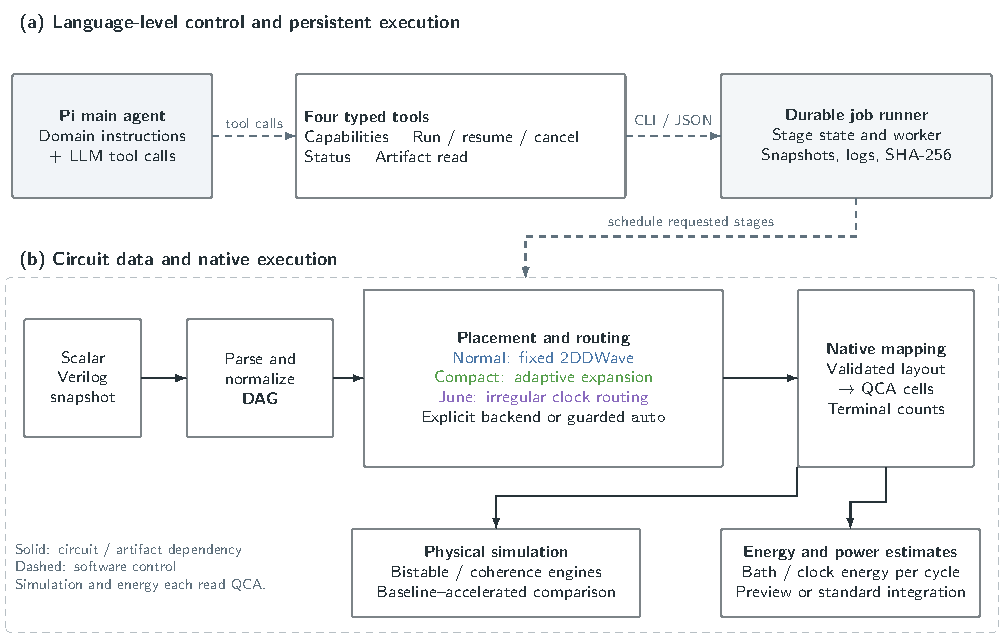
\includegraphics[width=170mm]{fig01_architecture.pdf}
\caption{FCNPilot design and control dependencies. The language agent selects a supported request; native design algorithms and deterministic checks produce the circuit evidence. Solid arrows denote circuit or artifact dependencies, and dashed arrows denote software control. Simulation and energy analysis both consume the mapped QCA device; energy analysis does not consume the numerical engine-comparison result. The lower dashed enclosure groups workflow stages and is not an interconnect. Diagram code was prepared with AI assistance from the implemented workflow.}
\label{fig:architecture}
\end{figure*}

\section{Background and Related Work}\label{sec:related}
\subsection{Clocked FCN physical design}
FCN physical design must accommodate connectivity and clocking together. Clock zones support directed information transfer, and their organization constrains where gates and interconnects can be placed. Two-dimensional wave clocking provides a regular spatial organization, whereas irregular assignments allow additional geometric freedom \cite{Vankamamidi2008Clocking}. Local phase compatibility, however, is not a substitute for reasoning about the arrival times of reconvergent signals.

Exact QCA placement and routing provides a reference for constraint-based design on tractable instances \cite{Walter2018ExactQCA}. Scalable approaches and sparsity-oriented or dedicated FCN placement-and-routing methods address larger search spaces and different layout objectives \cite{Walter2019ScalableFCN,Peng2021Spars,Li2022FCNPR}. The fiction framework provides an open environment for FCN design automation \cite{Walter2019Fiction}. Recent benchmark and design resources, including MNT Bench and MNT Designer, further support evaluation and access to emerging-technology design methods \cite{Hofmann2024MNTBench,Hofmann2025MNTDesigner}. These resources are relevant to future expansion of the present evaluation; their existence does not imply that their circuits have been validated by the restricted frontend studied here.

The published iFCN platform already includes circuit transformations, physical-design methods, QCA mapping, and physical simulation and energy-analysis capabilities \cite{Li2026iFCN}. Its graph-based methods, spatial data structures, routing procedures, and accelerated numerical routines are inherited foundations of this work. This paper assesses three executable backend paths from that platform and adds a language-facing decision layer with explicit acceptance and reporting conditions. It does not reattribute the underlying placement or simulation algorithms as new contributions.

\subsection{Verification and numerical analysis}
Formal verification of FCN circuits is an established research topic \cite{Walter2020Verification}. The exhaustive check used here addresses a narrower problem: whether the actual routed Boolean graph implements the supported scalar source under an explicit port correspondence. For small input counts, this offers complete input coverage without relying on a sampled test set. It does not model cell interactions, clocked transients, or device defects.

QCADesigner supports QCA circuit simulation, and energy-aware extensions enable investigation of energy dissipation under a physical model \cite{Walus2004QCADesigner,SillTorres2018Energy}. In such analyses, agreement between two implementations of a numerical engine is distinct from convergence to a physical solution. Similarly, a nonempty waveform file does not by itself show that output signals agree with the source truth table after the appropriate clock latency. These distinctions determine how simulation and energy results are interpreted below.

\subsection{Language-guided EDA}
ChatEDA studies LLM-assisted execution of EDA tasks through tool use \cite{Wu2024ChatEDA}. EDAid extends the investigation of agentic EDA workflows, while recent MCP4EDA and FluxEDA preprints explore related tool integration and agent-based design flows \cite{Wu2025EDAid,Wang2025MCP4EDA,Chen2026FluxEDA}. Thus neither natural-language access to EDA tools nor stateful orchestration alone is a sufficient novelty claim.

The specific issue studied here is the acceptance boundary for a QCA-oriented FCN flow: source semantics, routed geometry, and physical terminal counts can disagree even when individual programs complete. The proposed method makes these disagreements visible to the decision process. Its evaluation therefore reports both the circuit outcomes and the accuracy of the language agent's delivery. This also enables a fixed script to serve as a meaningful control: if the task specification is already structured, reliable deterministic execution may remain preferable.

\section{Circuit Representations and Acceptance Conditions}\label{sec:conditions}
\subsection{Scope and notation}
Let a source circuit be $S=(X,Y,\mathcal A)$, where $X$ and $Y$ are the explicitly declared input and output ports and $\mathcal A$ is a set of scalar continuous assignments. The supported expressions use complement, conjunction, disjunction, and exclusive OR. The current frontend handles a single combinational module; constants, buses, behavioral processes, hierarchy, and sequential elements are outside its accepted language. The target function is
\begin{equation}
F_S:\{0,1\}^{n}\longrightarrow\{0,1\}^{m},
\qquad n=|X|,\quad m=|Y|.
\end{equation}
Input and output order is fixed by the declared interface, not inferred from benchmark names.

A candidate produced by backend $j$ is represented as
\begin{equation}
c_j=(G_j,\rho_j,\mathcal R_j,\phi_j,Q_j),
\end{equation}
where $G_j=(V_j,E_j)$ is the actual routed directed acyclic graph (DAG), $\rho_j$ assigns graph nodes to integer grid positions, $\mathcal R_j$ contains the edge routes, $\phi_j$ assigns four-phase clock labels, and $Q_j$ is the mapped QCA cell collection. Technology decomposition and buffer insertion may change $G_j$ across backends. Checking only the initial parsed DAG would consequently leave a later transformation unexamined.

For an edge $e=(u,v)$, its route is a sequence $r_e=(p_0,\ldots,p_{\ell_e})$ connecting $\rho_j(u)$ and $\rho_j(v)$. Occupied gate-level area is measured by the bounding rectangle of all node and route coordinates:
\begin{equation}\label{eq:area}
A_{\mathrm{tile}}=(x_{\max}-x_{\min}+1)(y_{\max}-y_{\min}+1).
\end{equation}
This is a count of grid tiles. Device size is reported separately as $N_{\mathrm{cell}}=|Q_j|$, counting cell instances across all exported layers. Neither metric is a fabricated-device area, and a dimension such as $7\times8$ tiles must not be reported as $7\times8$ QCA cells.

\subsection{Geometry and local clock progression}
The geometric predicate $\mathcal G(c_j)$ collects the implemented structural and route checks. These include acyclicity, graph-node and edge coverage, unique gate locations, correct route endpoints, simple four-connected paths, exclusion of paths through unrelated gates, distinct input sides for a gate's fanins, and applicable crossing checks that distinguish separate signals. These are checks on the exported layout representation; they do not constitute a complete manufacturing rule set.

For each consecutive route pair, the common phase condition is
\begin{equation}\label{eq:clock}
\phi_j(p_i)\in\mathbb Z_4,\qquad
(\phi_j(p_{i+1})-\phi_j(p_i))\bmod4\in\{0,1\}.
\end{equation}
Thus a route may remain within a phase or advance by one phase. Normal additionally uses the fixed template $\phi(x,y)=(x+y)\bmod4$ and its directional input constraints. Compact and June use irregular phase assignments; the regular-template test is inapplicable to them. We denote the applicable backend-specific clock checks by $\mathcal C_j(c_j)$.

Equation~\eqref{eq:clock} carries no absolute cycle index. Two reconvergent paths can obey it without delivering corresponding input values in the same cycle. The reported maximum same-phase run is also not a common hard limit imposed on all three backends. Accordingly, $\mathcal C_j$ establishes the checked local progression conditions, not balanced latency or dynamic QCA correctness.

\subsection{Boolean correspondence and physical terminals}
Let $\beta_j$ bind source ports to ports of the routed graph. Input names must match explicitly, and output correspondence must follow exact names or an explicit pure-signal alias chain in the source. The checker requires an unambiguous output correspondence; it does not search for a permutation that happens to make truth tables agree. Unknown gate semantics, missing output labels, and ambiguous bindings yield an unsupported check, rather than an asserted Boolean counterexample.

For $1\leq n\leq11$, acceptance requires
\begin{equation}\label{eq:equivalence}
\mathcal E(S,G_j)=\mathrm{pass}
\ \Longleftrightarrow\ 
\forall x\in\{0,1\}^{n},\ F_S(x)=F_{G_j,\beta_j}(x).
\end{equation}
At most 2048 vectors are evaluated. Subject to correct expression and gate evaluators, this checks the complete combinational input domain. The corresponding evaluation cost is proportional to $2^n$ times the source and graph evaluation cost, motivating the explicit input limit. For larger designs, the current implementation may continue with a status that states the Boolean check was not performed because of this limit. An unsupported binding within the limit is rejected. All Boolean claims in this paper refer to candidates for which the check was actually performed.

Mapping introduces a different condition. Let $N_{\mathrm{in}}(Q_j)$ and $N_{\mathrm{out}}(Q_j)$ count the QCA cells tagged as input and output terminals. The interface-count predicate is
\begin{equation}\label{eq:terminals}
\mathcal I(c_j)=[|Q_j|>0]\land[N_{\mathrm{in}}(Q_j)=n]
\land[N_{\mathrm{out}}(Q_j)=m].
\end{equation}
It is deliberately weaker than source-to-device equivalence. Equal counts do not prove a bijection between named source signals and physical terminals, and do not establish the polarization at those terminals. Conversely, unequal counts identify a concrete loss of the declared interface even when Eq.~\eqref{eq:equivalence} passes.

Let $\mathcal M(c_j)$ denote successful native mapping and its applicable mapping/crossing checks, and let $\mathcal L(S,G_j)$ require either the Boolean pass in Eq.~\eqref{eq:equivalence} or the explicitly reported input-limit exemption. The production acceptance predicate is
\begin{equation}\label{eq:accept}
\mathcal A(S,c_j)=\mathcal G(c_j)\land\mathcal C_j(c_j)
\land\mathcal M(c_j)\land\mathcal I(c_j)\land\mathcal L(S,G_j).
\end{equation}
Each component is retained separately. This prevents the word ``validated'' from erasing which properties have been established. In the benchmark analysis, a \emph{qualified} execution specifically means that source-to-routed-DAG equivalence passes and mapped terminal counts match, in addition to its original execution checks; no input-limit exemption is counted as qualified.

\begin{figure*}[t]
\centering
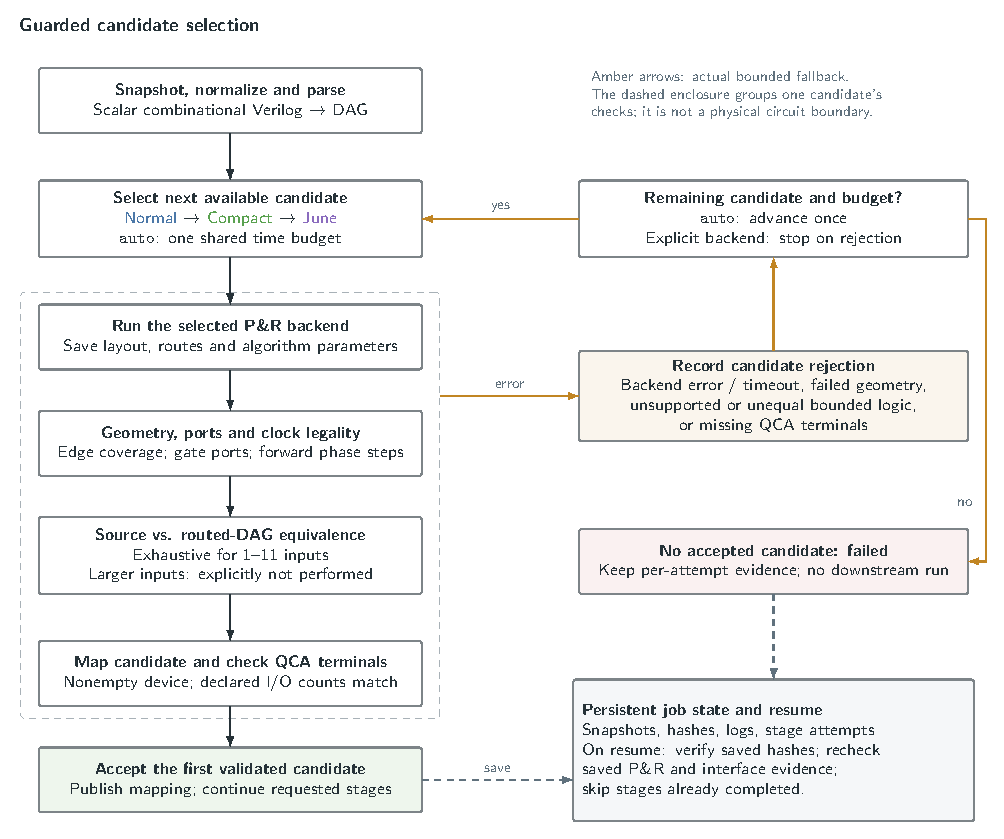
\includegraphics[width=170mm]{fig02_guarded_execution.pdf}
\caption{Candidate selection with explicit acceptance conditions. Each candidate is checked at the routed-graph and device-mapping boundaries. Automatic selection retains rejections and proceeds through the remaining backend sequence; explicit selection stops on failure. The first accepted candidate is returned. The shared routing budget controls external invocations and is not a hard deadline for the entire design flow. Above the 11-input Boolean limit, the unperformed check is reported explicitly. Figure code was prepared with AI assistance from recorded artifacts.}
\label{fig:selection}
\end{figure*}

\section{Language-Guided Candidate Selection}\label{sec:method}
\subsection{Separation of intent and acceptance}
The agent translates a request into a supported circuit source, desired endpoint, backend choice, and execution budget. It can request parsing alone, a mapped layout, or subsequent numerical analyses. It can inspect capabilities and read results when reporting to the user. Native design algorithms produce circuit coordinates, and deterministic checks decide acceptance. These outputs are not generated as free-form language. Figure~\ref{fig:architecture} shows this division.

The source used by a run is snapshotted before processing. Stage dependencies ensure that the mapped device corresponds to the selected routed candidate, and that numerical analyses consume that device. Stored hashes and immutable candidate records support this correspondence and allow an interrupted job to be inspected. They provide evidence of artifact identity, not a proof of circuit behavior. Resuming a completed routing or mapping stage requires its saved evidence to be rechecked.

This separation is also applied to the final report. The reported source, selected backend, occupied tiles, QCA cell count, and validation status must be read from the accepted result. A source/DAG Boolean pass cannot be paraphrased as physical verification. An iteration-limit warning remains attached to a simulation result even when a downstream stage completes. The pilot in Section~\ref{sec:pilot} examines whether an LLM actually respects these reporting requirements.

\subsection{Ordered backend portfolio}
The evaluated portfolio contains three existing physical-design paths. Normal combines graph-based placement and ordering with regular 2DDWave clocking. Compact uses a native compact-graph path with adaptive expansion and compaction. June uses its native placement-and-routing path with four-direction routes, post-route phase assignment, and buffer insertion. The names identify executable paths, not three newly proposed algorithms. Other methods present in the iFCN codebase are not included in this portfolio or its reported comparison.

Automatic selection visits the available backends in the fixed order Normal, Compact, and June. If $T$ is the shared routing-selection budget and $t_i$ is the elapsed selection time before candidate $i$, its external-call allowance is
\begin{equation}\label{eq:budget}
b_i=\max\!\left(1,\left\lfloor\frac{T-t_i}{K-i+1}\right\rfloor\right),
\end{equation}
provided at least one second remains; otherwise the unattempted candidate is recorded as budget exhausted. The candidate's remaining allowance is used for the QCA export probe after routing and logical checking. A failure, timeout, or failed predicate is retained before the next candidate is considered. An explicitly requested backend is not silently replaced, and cancellation terminates selection without fallback.

The first candidate satisfying Eq.~\eqref{eq:accept} is accepted. This is a first-feasible policy with a preference for the early backend, not area minimization or a learned portfolio policy. It avoids comparing an attractive but unqualified area against a qualified circuit. The initial order is a design choice; its general optimality is neither assumed nor demonstrated.

One invocation starts at most $K\leq3$ backend candidates because the finite list is traversed once and acceptance immediately exits the traversal. This bound does not extend across repeated user-initiated resumptions. Termination further assumes finite local validation and normal operating-system process termination. Local Boolean evaluation, hashing, and file processing are not independently preempted, and process termination includes polling and a grace interval. Consequently, $T$ is a shared routing budget with bounded external calls, not a hard real-time bound on either selection or the complete parse-to-energy flow.

\subsection{A design across representation boundaries}
Figure~\ref{fig:chain} follows a recorded XOR design. Its routed graph realizes $(a\lor b)\land\neg(a\land b)$, and all four input vectors agree with the source. The Normal layout occupies 12 tiles, whereas its device contains 79 QCA cell instances on three layers. This example illustrates why graph nodes, layout tiles, and physical cell instances must remain distinct quantities.

\begin{figure*}[p]
\centering
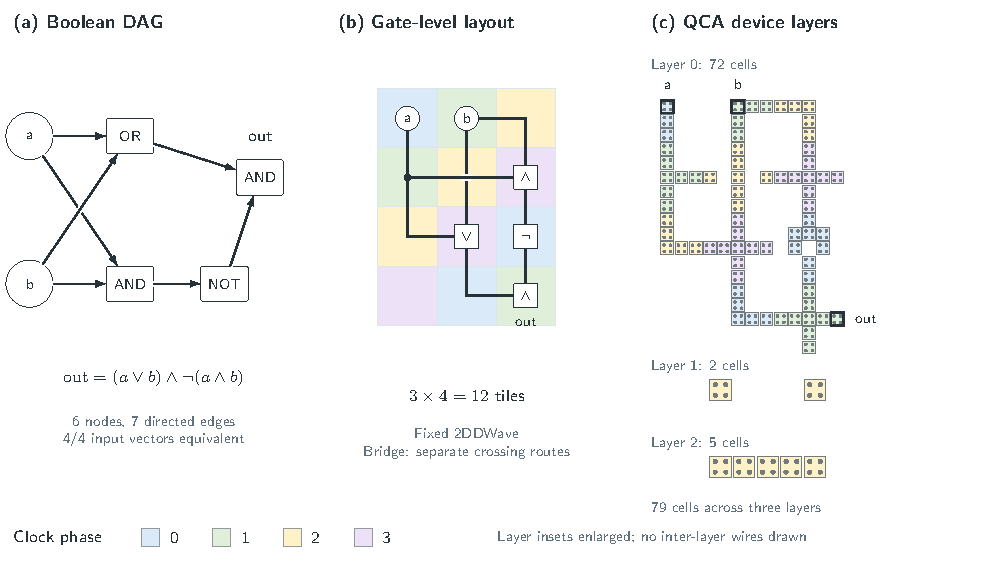
\includegraphics[width=170mm]{fig03_xor_design_chain.pdf}
\caption{One recorded Normal XOR design across representations: routed Boolean graph, clocked gate-level layout, and all mapped QCA cells separated by layer. The source/DAG check covers all four input vectors. The layout occupies 12 tiles and contains 79 QCA cells: 72, two, and five on layers 0, 1, and 2. Upper-layer insets are enlarged. Cell dots depict geometry, not simulated polarization; a graphical bridge denotes separate crossing routes. Figure code was prepared with AI assistance from recorded artifacts.}
\label{fig:chain}
\end{figure*}

Figure~\ref{fig:backends} shows the same frozen XOR source processed by the three backends. Normal and Compact export six-node, seven-edge graphs; June's routed graph contains three identity/wire nodes, yielding nine nodes and ten edges. Thus even a paired source comparison evaluates the complete backend paths. It cannot isolate the contribution of placement or routing on an identical optimized graph. The example is used to explain these representational differences, rather than to infer a general area ranking from one circuit.

\begin{figure*}[p]
\centering
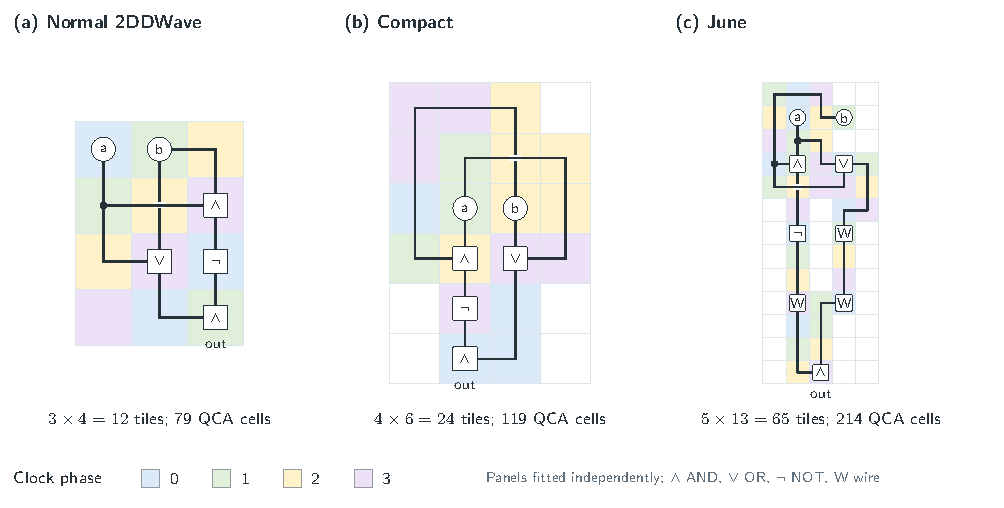
\includegraphics[width=170mm]{fig04_xor_backend_layouts.pdf}
\caption{Actual XOR layouts from Normal, Compact, and June. Bounding rectangles contain 12, 24, and 65 tiles; the devices contain 79, 119, and 214 QCA cell instances. Panels are fitted independently, so their displayed sizes are not area ratios. Colors show the exported zero-based clock phases; only Normal uses the fixed 2DDWave template. June includes buffer insertion and is taken from the separate 600-second-budget follow-up execution. Figure code was prepared with AI assistance from recorded artifacts.}
\label{fig:backends}
\end{figure*}

\section{Experimental Design}\label{sec:experiments}
\subsection{Frozen circuit corpus}
The corpus comprises 17 TOY and 13 MAJ source representations. Original source files are preserved; experiments use frozen copies with a manifest and content hashes. The 30 representations contain 29 byte-distinct files and 16 complete truth-table groups under fixed input and output declaration order. These are three descriptions of one corpus, not three successive filters. The grouping does not identify arbitrary port permutations or negation-permutation-negation equivalence. One representative of each group is fixed in the manifest before backend outcomes are selected.

Two curation changes are explicit. The TOY XOR module port header is normalized while retaining its logic. The frozen TOY two-bit ripple-carry adder is corrected to its declared addition interface and checked against an independent arithmetic reference on all 32 input vectors. The MAJ circuit with a similar adder name retains its original logic and is not assumed to be functionally matched. Other suggestive names are likewise not treated as specifications: the source named one-bit majority adder implements a single majority output rather than a complete full-adder interface.

All 30 frozen sources pass the recorded frontend checks and source-normalization equivalence tests; the additional parity canonicalization checks are also retained. These establish the input-processing scope, not the validity of every mapped device. Historical compaction tables with superseded legality assumptions, unvalidated larger-circuit results, and numerical-only comparisons are excluded from the present efficacy evidence.

\subsection{Three evidence cohorts}
Table~\ref{tab:cohorts} separates the experiments by question and implementation boundary. The 90-attempt backend matrix and the language-agent pilot were recorded before the later production acceptance guards. The additional logic and terminal-count audit is applied to the matrix's saved artifacts. Subsequent guarded regressions demonstrate specific acceptance and rejection behavior but do not constitute a rerun of all 90 attempts. Keeping these cohorts separate prevents a post hoc qualification count from being mistaken for the success rate of a newly guarded online workflow.

\begin{table*}[t]
\caption{Evidence cohorts and the conclusions they support. Every planned trial remains in its original denominator.}
\label{tab:cohorts}
\centering\small
\begin{tabular}{@{}>{\raggedright\arraybackslash}p{29mm}>{\raggedright\arraybackslash}p{37mm}>{\raggedright\arraybackslash}p{46mm}>{\raggedright\arraybackslash}p{49mm}@{}}
\toprule
Cohort & Design & Principal measurement & Interpretation boundary\\
\midrule
Archived backend matrix & 30 representations $\times$ 3 explicit backends; 90 attempts & Original execution completion, followed by independent DAG and terminal-count audits & The qualified count is retrospective; automatic fallback was not measured in this matrix.\\
Language-agent pilot & Four task types $\times$ two repeats $\times$ three methods; 24 trials & Mapping execution and prespecified task delivery, plus a separate text audit & Uses the archived workflow; tasks end at mapping and do not test simulation or energy analysis.\\
Later guarded executions & Two diagnostic circuits and three XOR full-flow cases & Candidate rejection/recovery, exported interfaces, numerical-stage completion & Targeted cases validate implemented behavior; they do not estimate general coverage or physical correctness.\\
\bottomrule
\end{tabular}
\end{table*}

Each matrix attempt explicitly selects one backend and targets device mapping, with a 180-second per-command timeout, two concurrent workers, and one attempt without retry. Inputs and relevant executable/source identities are preserved in the records. A requested seed of one does not fully control native backend randomness because the native internal seed is not exposed. The matrix therefore describes the observed runs; it is not a multi-seed estimate of search reliability.

Coverage is first reported over all representations, then over the preselected function representatives. A failed representative is not replaced by a successful equivalent alternative. Paired area observations use only representatives qualified by both backends in a pair, with area independently recomputed by Eq.~\eqref{eq:area}. Different pairs have different common-case sets. Unpaired means and missing failures are not used to claim an area improvement.

For the pilot, the fixed script receives structured task fields, including an explicitly supplied recovery alternative. Generic Pi and the domain agent use the same \texttt{qwen3-vl-plus} model, tools, task prompts, permissions, backend parameters, and budgets; their system prompts differ. The four tasks concern ordinary mapping, selecting a specified backend, recovering from a missing input using a supplied alternative, and reporting metrics and validation boundaries from artifacts. Each has two independent session repeats per method. Trials use a 180-second allowance, at most 12 tool calls, a 3500-output-token limit, and a 90-second backend setting. Trial order is shuffled and two sessions run concurrently. This small controlled pilot evaluates delivery under the recorded service conditions, not general reasoning ability.

\subsection{Analysis and figure preparation}
OpenAI Codex assisted in organizing literature, preparing scripts that aggregate the recorded outcomes, drafting the manuscript, and writing TikZ figure code. This preparation is distinct from the real-model pilot. Numerical summaries were checked against the saved per-run records, and source, layout, and device identities were checked through their stored hashes. Circuit drawings use exported coordinates; plots use recorded trial outcomes or numerical samples. No synthetic benchmark measurements, generated polarization traces, or invented experimental successes are introduced by the drafting process.

\section{Results}\label{sec:results}
\subsection{Execution completion and qualified coverage}
Under the original matrix execution criterion, Normal, Compact, and June complete 21, 10, and 24 of 30 attempts, respectively, for 55 of 90 in total. Auditing those 55 routed graphs establishes source equivalence in 51 cases and an unsupported binding or interpretation in four; no audited case is established to be nonequivalent. The completed equivalence evaluations cover 9280 input vectors in aggregate. Separately, four mapped devices have incorrect output terminal counts, with one case overlapping the unsupported-DAG set. Therefore seven distinct execution completions fail the added qualification conditions, leaving 48 qualified attempts, or 53.3\% of all planned attempts.

Figure~\ref{fig:coverage} retains the complete matrix. The decrease from 55 to 48 shows why execution completion overstates the checked result: 12.7\% of the original completions lack either established source/DAG equivalence or the required terminal counts. This is not a measured physical error rate. In particular, an unsupported Boolean audit is an evidence gap, not a demonstrated logical mismatch.

Of the 35 incomplete attempts, 22 are rejected by route or phase checks, three by repeated-crossing checks for a same-source routing-tree pair, nine do not produce a complete legal layout, and one times out in routing. Thus incomplete execution combines constraint violations and search failure; it is not a homogeneous set of Boolean errors. Among the seven later-disqualified completions, three fail only the supported-DAG requirement, three fail only terminal counts, and one fails both.

\begin{figure*}[t]
\centering
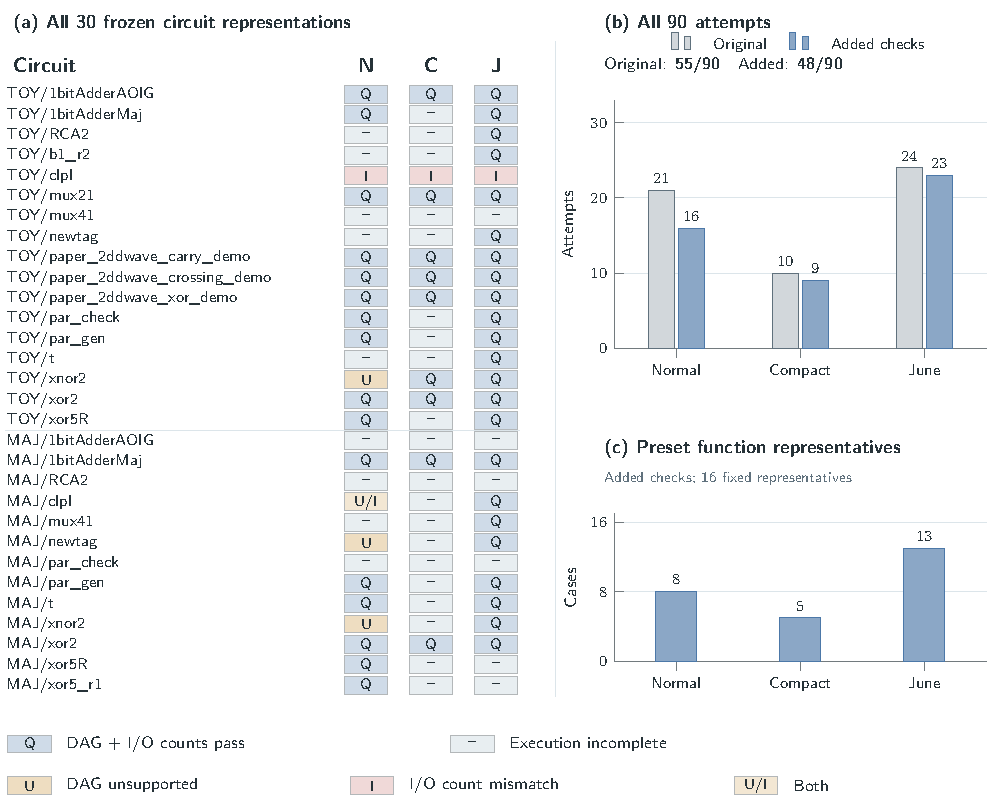
\includegraphics[width=170mm]{fig05_backend_coverage.pdf}
\caption{All 90 archived backend attempts and their retrospective qualification. Q denotes a completed execution with source/DAG equivalence and matching QCA terminal counts; U denotes an unsupported DAG audit, I a terminal-count mismatch, U/I both, and a dash incomplete execution. Original completions total 55; adding the independent checks leaves 48. On the 16 representatives fixed in advance, qualified counts are 8, 5, and 13. These outcomes precede the later production guards and do not establish device waveform correctness. Figure code was prepared with AI assistance from recorded artifacts.}
\label{fig:coverage}
\end{figure*}

Table~\ref{tab:coverage} gives the corpus breakdown. Across all 30 representations, the qualified backend sets have a union of 25 and a three-way intersection of eight. That union is an observed availability set, not an automatic-selector success rate. More importantly, the union on the 16 fixed representatives contains 13 functions, equal to June's qualified count, and the three-way intersection contains four. The present function-level evidence therefore does not show a coverage gain from combining all three backends over June alone. The portfolio can still encode a preference for an earlier qualified layout, but that policy benefit must not be conflated with expanded functional coverage.

\begin{table}[!ht]
\caption{Completed/qualified counts by source group. The representative set is fixed before selecting outcomes.}
\label{tab:coverage}
\centering\small
\begin{tabular}{@{}lrrr@{}}
\toprule
Corpus & Normal & Compact & June\\
\midrule
TOY ($17$) & 12/10 & 8/7 & 16/15\\
MAJ ($13$) & 9/6 & 2/2 & 8/8\\
All representations ($30$) & 21/16 & 10/9 & 24/23\\
Fixed representatives ($16$) & 10/8 & 6/5 & 14/13\\
\bottomrule
\end{tabular}
\end{table}

Alternative representations matter. Selecting any successful equivalent representation after observing the outcomes would raise availability to 15 of the 16 truth-table groups, but this is a different, post hoc criterion. It is not substituted for the 13-of-16 preselected-representative result. This distinction exposes sensitivity to circuit representation without crediting additional files as independent functions.

\subsection{Occupied area on common qualified cases}
The three paired comparisons contain four Normal--Compact, eight Normal--June, and five Compact--June representatives. Their arithmetic mean occupied areas are 22.5 versus 43.5, 55.25 versus 342.625, and 44.4 versus 116.8 tiles, respectively. Figure~\ref{fig:area} displays the individual observations rather than presenting these means as a single ranking over a common population.

\begin{figure*}[t]
\centering
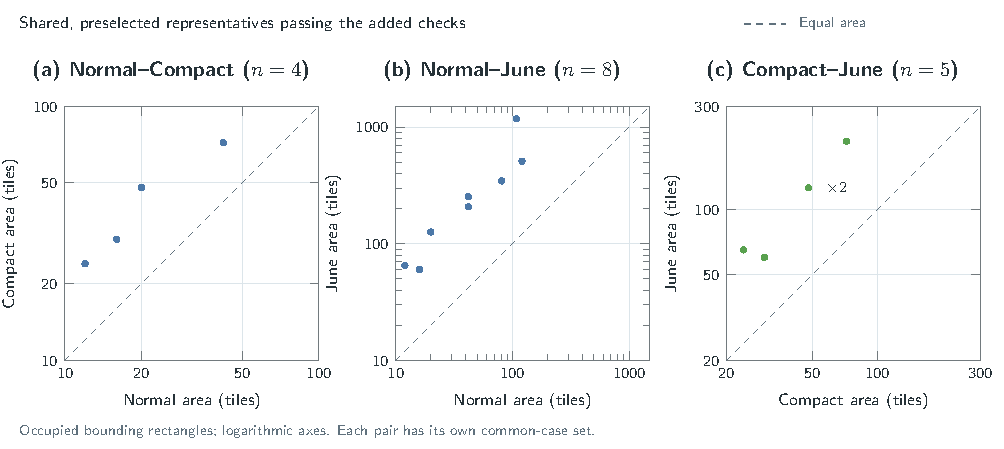
\includegraphics[width=170mm]{fig06_paired_area.pdf}
\caption{Occupied-area pairs for preselected representatives qualified by both backends in each panel. Areas are recomputed from all gate and route coordinates in tiles; the dashed line denotes equality. Logarithmic axes have matching limits within each panel. The pairwise cohorts contain four, eight, and five representatives and are not interchangeable. Two Compact--June observations coincide at $(48,126)$ and are marked with multiplicity two. A shared source does not imply an identical internal DAG. Figure code was prepared with AI assistance from recorded artifacts.}
\label{fig:area}
\end{figure*}

The observed means motivate retaining a compact early candidate when it qualifies, while the coverage results motivate trying another backend when it does not. They do not establish optimality of the chosen order. Common-case selection excludes failures by construction, the number of distinct functions is small, and backend-specific graph transformations contribute to the measured area. A direct algorithmic comparison would require matched intermediate graphs, controlled native randomness, and an explicit treatment of infeasible instances. Device-cell area and clock-latency performance would also require separate measurements.

\subsection{Language-agent delivery}\label{sec:pilot}
Figure~\ref{fig:pilot} separates mapping execution from task delivery. The fixed script, generic Pi, and domain agent complete mapping in 8/8, 7/8, and 6/8 trials, respectively. Under the prespecified structured-delivery criterion, their scores are 8/8, 5/8, and 6/8. A subsequent audit of free-text claims gives 8/8, 5/8, and 5/8 when added to the original delivery requirements. The post hoc criterion is reported separately and does not replace the prespecified score.

\begin{figure*}[t]
\centering
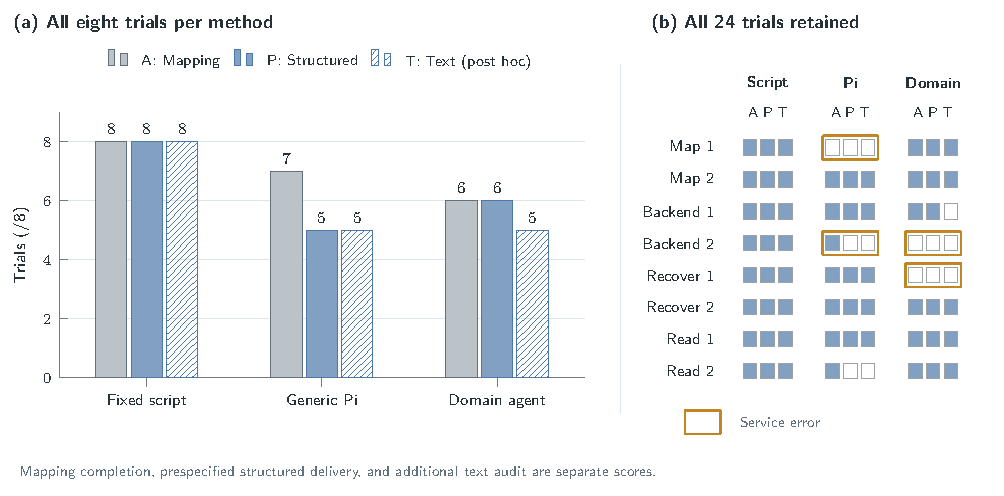
\includegraphics[width=170mm]{fig07_llm_pilot.pdf}
\caption{Pilot outcomes for eight trials per method, retaining all 24 trials. A denotes mapping execution under the archived criterion, P prespecified structured delivery, and T the additional post hoc text audit. Every trial is shown in the right-hand panel. Amber outlines identify provider/service errors, including one generic-Pi trial that mapped successfully before delivery failed. The two language conditions share the model, tools, and budgets; the fixed script uses structured specifications. The pilot ends at mapping and supports no general superiority claim. Plotting code was prepared with AI assistance from recorded outcomes.}
\label{fig:pilot}
\end{figure*}

Each LLM condition encounters one connection error and one account-state refusal. These four service-affected trials remain in the denominators. In one generic-Pi trial, mapping finishes before the connection failure prevents delivery, explaining why tool completion and delivered success differ. Removing such trials after observing the results would answer a different question about availability and would change the small sample materially.

Content errors are also informative. Generic Pi cites a source artifact that does not contain every reported metric, including a cell count it does report correctly. In one domain-agent report, $7\times8$ gate-level tiles are described as cells even though the mapped device contains 258 cells. That report passes the structured criterion but fails the additional text audit. No trial falsely claims that an unfinished run completed, yet the unit error shows that accurate completion status is insufficient for a scientifically correct report.

The pilot provides no reliable evidence that the domain agent outperforms generic Pi, and the fixed script delivers all eight structured tasks. The single-trial difference between the LLM conditions is too fragile for a superiority claim, especially given service failures and only four task types. The domain prompt was subsequently strengthened to emphasize source identity and metric units; no new real-model pilot has validated that revision. The defensible result is feasibility of language-mediated access with measurable reporting failure modes, rather than demonstrated productivity or correctness gains from the LLM.

\subsection{Recovery and loss of physical outputs}
The later guarded executions reveal two distinct failure mechanisms in circuits with 11 inputs and five outputs (Figure~\ref{fig:recovery}). For MAJ/clpl, Normal cannot establish an explicit binding for source output $y_0$ and is rejected as unsupported. Compact exceeds its 77-second native routing allowance. June then passes all 2048 source/DAG vectors and preserves 11 input and five output terminals, so the candidate is accepted through mapping. This is a recorded recovery within one ordered selection, not an estimate of its probability of success.

\begin{figure*}[t]
\centering
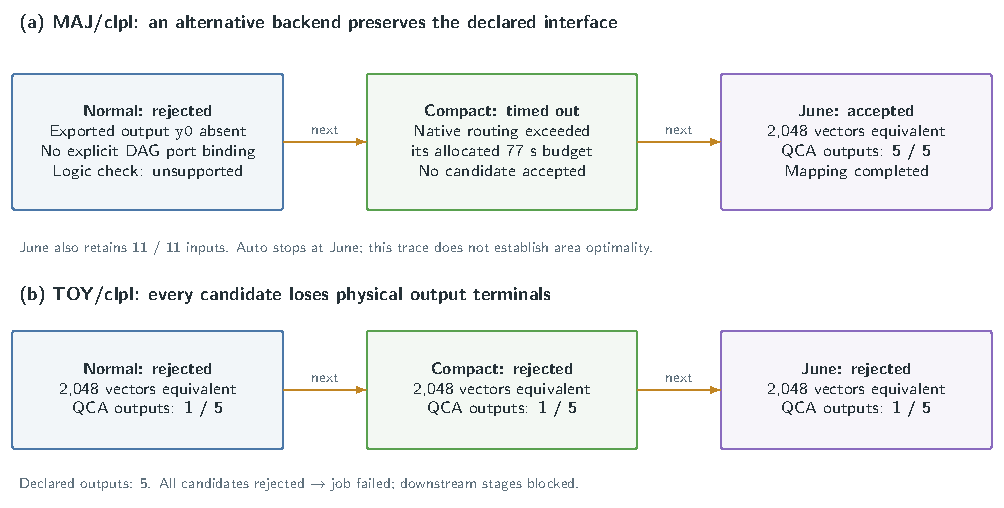
\includegraphics[width=170mm]{fig08_failure_recovery.pdf}
\caption{Two later production traces. For MAJ/clpl, an unsupported Normal output binding and a Compact timeout precede a June candidate that passes 2048 Boolean vectors and preserves all terminal counts. For TOY/clpl, all three DAGs pass 2048 vectors, but every device exposes only one of five declared outputs; all candidates are rejected. Fractions show observed/declared terminals. These are two recorded executions, not probabilities or device-function proofs. Figure code was prepared with AI assistance from recorded artifacts.}
\label{fig:recovery}
\end{figure*}

For TOY/clpl, all three routed graphs are Boolean-equivalent to the source over the same 2048 vectors. Nevertheless, every device export exposes only one of the five declared outputs. All candidates are rejected before downstream analysis. Inspection of the mapping implementation provides a mechanism for this discrepancy: output-cell generation in some gate templates depends on whether the gate has successors. A logical node that is both externally observed and internally consumed can therefore require an output realization that the chosen template does not preserve.

This case establishes a concrete separation between static function preservation and preservation of physical output observability. A Boolean check alone would not catch it, while counting terminals cannot replace the Boolean check in the first case. The present contribution detects and contains these failures; it does not repair all affected mapping templates or prove the behavior of the accepted device.

\subsection{Full-flow numerical case study}\label{sec:numerical}
Later executions take the same frozen XOR source through each backend, device mapping, Bistable and Coherence engine comparisons, and standard energy analysis. Normal completes in 99.804~s. Compact completes with warnings in 135.453~s, including seven Bistable iteration-limit samples. June's initial 180-second energy invocation times out; a separately recorded run with a 600-second allowance completes in 238.944~s overall. The three completed examples consequently do not constitute uniform-budget success or an LLM-controlled full-flow benchmark.

For the Normal device in Figure~\ref{fig:chain}, the baseline and accelerated exported outputs coincide for all 512 retained Bistable samples and all 3005 retained Coherence samples. Figure~\ref{fig:numerical} shows the traces without alignment or smoothing. This is numerical implementation agreement on a recorded device. The comparison does not align device outputs to source input vectors and therefore does not establish source-to-device functional equivalence.

\begin{figure*}[t]
\centering
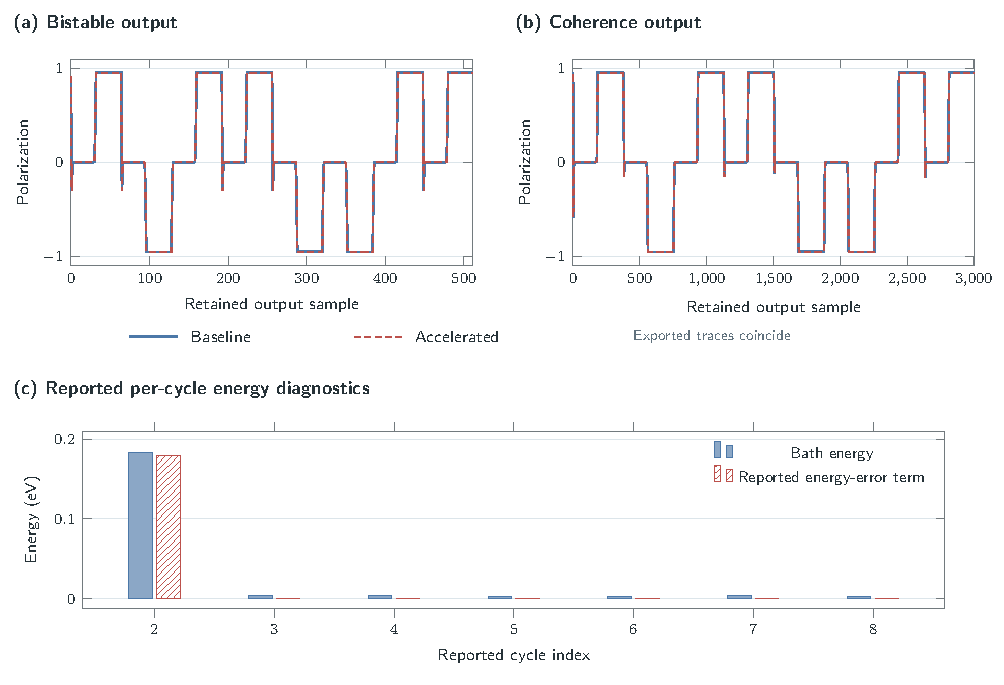
\includegraphics[width=170mm]{figS2_numerical_diagnostics.pdf}
\caption{Numerical diagnostics for the Normal XOR device in Figure~\ref{fig:chain}. All 512 Bistable and 3005 retained Coherence output samples are shown without temporal alignment, interpolation, or smoothing. Coincident baseline and accelerated traces establish implementation agreement, not source-to-device correctness. All seven reported energy cycles are included; the energy-error field is a numerical diagnostic rather than a statistical error bar. The energy and Coherence steps are $10^{-17}$ and $10^{-16}$~s, respectively. No time-step or steady-state convergence is established. Plotting code was prepared with AI assistance from recorded data.}
\label{fig:numerical}
\end{figure*}

The standard energy run uses a $10^{-17}$~s step, while the displayed Coherence comparison uses $10^{-16}$~s. All seven reported energy cycles are retained. The total reported bath energy is $0.202920$~eV and the summed reported energy-error field is $0.179718$~eV; the first reported cycle contributes most of the latter. The average bath energy is $0.0289886$~eV per counted cycle. With the configured $10^{-11}$~s period, this corresponds arithmetically to approximately $4.64\times10^{-10}$~W in the model. The large diagnostic term and absence of a time-step or steady-state study prevent interpreting that value as an accurate dissipation estimate or an energy-saving result. Numerical completion makes these diagnostics available for scrutiny; it does not remove their limitations.

\section{Discussion}\label{sec:discussion}
\subsection{What the evidence establishes}
The strongest empirical result is the separation of acceptance conditions at different circuit representations. Seven of 55 archived execution completions fail the additional qualification requirements, and a later case demonstrates a Boolean-equivalent graph with a deficient physical output interface. This gives the acceptance conditions a circuit-specific role beyond general workflow error handling. Retaining unsupported and rejected outcomes also prevents attractive area measurements from obscuring an unestablished circuit property.

The portfolio provides a controlled way to use the existing diversity of implementations. A candidate can be rejected for one representation failure and another backend can produce a qualifying result, as in the MAJ/clpl trace. However, the fixed-representative matrix does not show coverage beyond June's 13 qualified functions. The evidence supports conditional recovery and differing observed area/coverage behavior, rather than a general gain from portfolio selection.

The LLM layer adds an interface for specifying and inspecting this process. It is not the source of the circuit correctness evidence. Indeed, the pilot's reporting errors and the deterministic baseline's success indicate that a language interface should remain accountable to machine-readable measurements. A useful subsequent study would vary task ambiguity and the need for adaptive reasoning while retaining the same deterministic checks and a properly specified script baseline. The current pilot is too small to determine where that additional flexibility becomes beneficial.

\subsection{Validity and extension}
The 30 representations correspond to only 16 fixed-order truth-table groups, and the evaluated language is a restricted scalar combinational subset. Repeated representations, native search randomness, backend-specific DAG transformations, and small common-case sets limit generalization. The archived matrix, later guards, and post-pilot prompt revision are distinct implementation states. Their results must not be pooled into a single latest-system success rate.

Three verification gaps remain consequential. Above 11 inputs, source/DAG equivalence is not established by the present exhaustive checker; a scalable formal method is needed before claiming the same logical coverage. At the mapping boundary, terminal counts should be extended to named signal correspondence and explicit realization of observed internal nodes. At the physical boundary, checking local phase progression should be complemented by latency-aware input/output testing and, where feasible, stronger device-level verification. These additions would strengthen different predicates rather than merely increase the number of successful tool calls.

Sequential extension requires a separate semantic model with state, initialization, and time-dependent observations. A sequential circuit cannot be validated by treating its signals as another combinational truth table. The architecture retains an extension point, but no sequential physical-design or verification result is claimed here. Broader combinational benchmarks, repeated controlled backend runs, and convergence studies should precede stronger claims about scalability, area efficiency, or power accuracy.

\section{Conclusion}\label{sec:conclusion}
This work presents a language-guided FCN design flow in which candidate acceptance is determined by explicit circuit checks. The method connects the existing iFCN transformations through Pi while distinguishing routed-graph equivalence, geometric and local clock conditions, QCA terminal counts, and numerical analysis. On a frozen 90-attempt matrix, independent logic and terminal-count audits reduce 55 execution completions to 48 qualified outcomes. Later guarded traces demonstrate both recovery and rejection of a mapping that loses required outputs.

The results support a reproducible small-combinational design study with inspectable acceptance boundaries. They do not establish device-level functional correctness, a general coverage advantage from the backend portfolio, or superior delivery by the language agent. The main research direction is to extend the same explicit treatment of evidence to named physical terminals, latency-aware device behavior, and larger or sequential circuits.

\section*{Data Availability Statement}
The supporting data comprise the frozen TOY/MAJ inputs and manifest, recorded backend and agent-trial outcomes, layout and device artifacts, and numerical traces retained in the FCNPilot repository under \texttt{engine/tests/benchmarks\_pi/} and \texttt{experiments/archive/}. The records preserve source identities and distinguish the archived experiments from later guarded executions. No public accession has been assigned to this experimental dataset.

\section*{Acknowledgments}
Generative AI assistance was used in manuscript drafting and editorial checks. Its use in literature organization, analysis-code preparation, and figure-code preparation is described in Section~\ref{sec:experiments}. The figures derive from recorded circuit artifacts and numerical data. No claim of scientific validity rests on language-model output alone.

\bibliography{references}
\end{document}
